
\label{chapter:cranfield}

Often, when I talk about search engines and how to build them, these
ubiquitous portals to the Internet—whether you’re using Bing, Yahoo!,
Baidu, or Ask Jeeves—seem like a fundamental law of science.
%
With the onslaught of \abr{ai}, they almost seem antiquated\dots my
parents use Google, but I use Grok.
%
But it wasn’t always like that: there was a time before search
engines, and although there’s a certain charm to card catalogs, that’s
not an effective way to find information.
%
But that was essentially the world before search engines: you had to
find what you wanted from a list or index.

My goal in this video is to tell the story of the Cranfield paradigm
and how it made the twentieth century Internet possible.
%
Most of this is drawn from the article ``The Evolution of Cranfield''
by~\citet{voorhees-19}, which I encourage you to read something with
more detail and more references, more focused on information
retrieval.

The story begins in 1967 with Cyril Cleverdon at Cranfield University
in England: which has an airport right on campus.\footnote{Here
at the University of Maryland we have to walk a whole fifteen minutes
to get to the oldest continuously operated airport in the world.}
%
The University was the heart of British aviation research.
%
Cyril Cleverdon was in charge of their library there.  And he was big
into computers.  He wanted to see if he could measure how good an
index was.

\begin{figure}
  \includegraphics[width=\textwidth]{figures/external/Cranfield_Airport_by_Thomas_Nugent}

  \caption{Photo of Cranfield University (and its adjacent airstrip).
    Photo by Thomas Nugent [Creative Commons Attribution-ShareAlike
    2.0 license].}
\end{figure}

Now, when I say ``index'', if you're over 40, you might think of this
sort of thing in the back of a book~\citep{ritchie88}:
\begin{quote}
  \begin{flushright}
    \flushright INDEX 269
    \end{flushright}

  
  \texttt{read} system call \hphantom{\dots} 170 \\
  \texttt{readdir} function \hphantom{\dots} 170 \\
  \texttt{readlines} function \hphantom{\dots} 170 \\
  \texttt{realloc} library function \hphantom{\dots} 170 \\
  recursion 86, 139, 141, 182, 269
\end{quote}
An author carefully wrote down topics mentioned in a text and told you
where you could find them (i.e., which page of the book they were
on).\footnote{In this case, they also helpfully told you that
  ``recursion'' appeared in the index (the page you're looking at), a
  computer science joke.}

But if you’re younger and a computer scientist, you probably think of
an index as a lookup table of every darn word possible.
%
The reason you think that is because of the Cranfield experiments.
%
His claim, which was quite controversial at the time, was that you
could look up documents based on the words in the document.
%
You didn’t need laboriously curated indices you could use a machine,
an engine if you will, to search through them.
%
The claim was that the Universal Decimal Classification, a facet
classification, and alphabetical subject catalog, and a unigram index
were roughly comparable~\cite{cleverdon-67}.

Before we analyze this, just a reminder of how a search engine query
is evaluated.  Again, this is old hat now but was revolutionary at the
time.  To evaluate a system’s ability to search a dataset, you take
some queries from users and then find the truly relevant documents to
that query.  Then, given a system’s results, you compute the
precision—out of all of the documents they returned how many were
right—and recall—out of all possible right documents how many did they
find.

Because these concepts are important, let's pause to review how
success at finding a relevant answer was measured by \citet{keen-66}.
%
First let's consider---given a query---how many answers you
retrieved.
%
Some of those were relevant to the query and gave you information you
wanted.  Let's say there are $A$ of those.  But others were not
relevant, these are distractions that you still have to weigh
through.  Let's say there are $B$ of those.

\begin{table}
\centering
\begin{tabular}{lccc}
\toprule
 & \textbf{Relevant} & \textbf{Non-relevant} & \textbf{Total} \\
\midrule
\textbf{Retrieved} 
    & $A_q$ 
    & $B_q$ 
    & $A_q + B_q$ \\
\textbf{Not Retrieved} 
    & $C_q$ 
    & $D_q$ 
    & $C_q + D_q$ \\
\midrule
\textbf{Total} 
    & $A_q + C_q$ 
    & $B_q + D_q$ 
    & $A_q + B_q + C_q + D_q$ \\
\bottomrule
\end{tabular}
\caption{Contingency table for question $q$ used to define precision
  and recall.}
\end{table}

Clearly it's better to have $A$ be higher than $B$, and this metric is
called \emph{precision}:
\begin{equation}
  \mbox{precision}(q) = \frac{A_q}{A_q + B_q},
\end{equation}
of the answers you provided, how many were relevant.  The higher the
better.
%
But let's consider how many of the relevant answers you did find:
$A_q$.  It would be better if $A_q$ were \emph{all} the relevant
documents, of which there are $A_q$ and $C_q$.
%
This is called the recall:
\begin{equation}
  \mbox{recall}(q) = \frac{A_q}{A_q + C_q}.
\end{equation}
Both of these numbers are between 0 (bad) and 1 (good); ideally, you
would want both to be 1.0, but this is hard to achieve.
%
You can get perfect recall by returning all possible answers, but then
your precision sinks.
%
If you return only the answers you're absolutely certain of, your
recall suffers.

Different applications (or users) would have different tradeoffs.
%
If you're trying to find a ``smoking gun'' in a court case, you want
recall over all else: it doesn't matter if you have to comb through
too many irrelevant documents.
%
But if you're trying to answer a simple question, you don't need every
document that tells you what the capital of Arkansas is, you just need
one, and you don't want anything irrelevant.


Let’s pause for a moment to recognize how revolutionary this was.  Once you found the relevant documents, you can evaluate *any* system.  Before, you had to run an expensive user experiment every time you tweaked your system: did that output look good?  How about this one.  With a reusable test collection, you could turn the crank on your retrieval system without pesky humans getting in the way.  Just check whether the red box finds the relevant documents!

But not everybody was convinced.  The Cranfield paradigm is making a lot of assumptions here: 
first, if a document is relevant, it’s equally relevant: everything is equally relevant: showing you my explanation of topic modeling is as good as a video from Siraj Raval’s
The users’ information needs are static; the answer to the question
``who is the president of the united states'' never changes (Nixon is
still president, right?).
%
Finally, the Cranfield paradigm assumes that somebody, somehow can
find the right answer from thousands or millions of documents.

The academic community at the time was skeptical.  There’s no way
these newfangled search engines could be better than a trained
librarian armed with a card catalog!
And \citet{cuadra-68} noted reasonable criticisms: different users have
different information needs---I don't need anybody to tell me what the
capital of Maryland is, but I don't know the capital of the
Yevreyskaya Oblast; the same user has different needs---I might do the
same search twice to get the citation for Cuadra and to find a good
quote.
%
And Cuadra does have some good quotes, he correctly warns us:
\begin{quote}
  For a time, psychologists devoted their attention
not to what was important, but to what was measurable. This is a surefire
approach to a certain kind of respectability, which information
scientists now desire as much as psychologists did then, but it risks
losing the baby with the bathwater. 
\end{quote}

Despite all those flaws, the assumptions—on average—mostly hold.
%
That’s why we’re still talking about the Cranfield paradigm fifty
years later.
%
And there were some big additions to the Cranfield
paradigm.
%
Most prominent was the use of better document representations and
creating larger test collections, which was spearheaded by Karen
Sp\"ark Jones a little bit west of Cranfield at Cambridge and by Ellen
Vorhees and others at the National Institute for Standards and
Technology in Gaithersburg, Maryland.

\subsection{Term-Frequency and Inverse Document Frequency}
\label{sec:ir:tf-idf}

We will talk about neural representations later when we talk about
models like \abr{bert} (Section~\ref{}).
%
Those representations are called \emph{dense}---not because they're
dumb, they're quite clever---but they packe a lot of information into
a small packet of computer memory.
%
In contrast, the representations that Karen Sp\"ark Jones came up with
are \emph{sparse}: they could have an entry for every word in your
language, but for any given question, you're only going to have a
handful of words present.

And because ``word'' is ambiguous, we'll call this ``term frequency''
instead.
%
The entry for a question has a higher weight for a word the more often
it appears.
%
E.g., if the question is:
\question{Which of the members of Lincoln's cabinent did Licoln previously serve in the House of Representative with?}
then the words that appear most commonly are going to be more important.
%
In this case, that would be ``Lincoln'' 

These took the theoretical insights of the original
Cranfield experiments and made them into something that could actually
work.  Again, this was revolutionary: as a result the British
Computing Society named their annual award for researchers in this
area after Karen Spärk Jones.

\section{Old-Fashioned \abr{ai}}
\label{sec:ir:gofai-qa}

Given the Cranfield paradigm, we now have a setup for creating \abr{qa}
system.
%
Build a collection of questions and see how well you can answer them.
%
And this defined how computers answered questions in the mid twentieth
century.\footnote{This is sometimes called ``good ol' fashioned \abr{ai}'' or
  \abr{gofai} for short.}

The history of question answering begins with
answering questions about the American sport
of baseball.
%
Since one of my big interests is comparing human vs. computer ability, it's
worth comparing it to the state of the art in human question
answering in the mid-twentieth century~\cite{sedman-11}:
\begin{quote}
Abbott: Goofy, huh? Now let's see. We have on the bags - we have Who's on first,
What's on second, I Don't Know's on third. \\
Costello: That's what I wanna find out. \\
Abbott: I say Who's on first, What's on second, I Don't Know's on
third--- \\
Costello: You know the fellows' names? \\
Abbott: Certainly! \\
Costello: Well then who's on first? \\
Abbott: Yes! \\
Costello: I mean the fellow's name! \\
Abbott: Who! \\
Costello: The guy on first! \\
Abbott: Who! \\
Costello: The first baseman! \\
Abbott: Who! \\
Costello: The guy playing first! \\
Abbott: Who is on first! \\
Costello: Now whaddya askin' me for? \\
Abbott: I'm telling you Who is on first. \citep[pages 1002--1004]{light-16}
\end{quote}

That’s going to be tough to beat.
Let’s take a look at the BASEBALL system
from MIT.
%
Despite the odd phrasing, the BASEBALL system
of Green et al. is essentially a natural language
interface to an existing database.

It does this by taking each word in the question,
trying to match it to a field in its database.
%
The the challenge then is to figure out what
the question is looking for, which is usually
%
found in the question word (this is quite a bit simpler than the lexical
answer type analysis of the Watson system
(Chapter~\ref{sec:watson:feature-engineering}), where you need to figure out
things like ``This Argentenian Author'' could be Borges, Cortazar, or Puig).

But if you know a database language like SQL,
you recognize that this is essentially a bunch
of SELECTs and WHEREs.
%
This isn’t even taxing the full breadth
of SQL.
%
To go the next step, we turn to a system called
LUNAR.

Which, as you might guess, was about the moon.
%
It could answer much more complicated questions,
such as those that require averages or averages
%
filtered by some criterion.
%
It can do this by converting the questions
into a rich, recursive grammar.
%
But first, it needs to analyze the grammatical
structure of the input question.

For example, the question “what is the average
modal plagioclase concentration for lunar
%
samples that contain rubidium?” is analyzed
with the following parts of speech.
%
Notice that it’s important to detect things
like relative clauses, which restrict the
%
level of analysis.

\jbgcomment{Need a figure for this}

After that syntactic analysis, it then gets
turned into a logical form that can be executed
%
against its database.

In 2022, it’s probably not worth going into
that.

Our databases don’t look like this anymore.
%
One thing that I found interesting in rereading
this in the perspective of the 21st century,
%
is that it also has something that looks like
an IR component, although it’s explicitly
%
looking for documents tagged with a particular
topic, unlike doing something like tf-idf
%
retrieval.

The last old school QA system I wanted to
talk about is probably the most famous of
%
them all: SHRLDU.
%
SHRDLU was described in the thesis of Terry
Winograd\dots remember that name, we’ll be
%
seeing it again!

Unlike the LUNAR and BASEBALL which are exactly
what they say on the tin, I need to explain
%
the name a little bit more.
%
This isn’t going to be easy.

First, since you’re reading a book printed in the twenty-first century,
you probably don’t know what a linotype
system is.
%
It was the “missing link” between moveable
type presses (where you had to move the letters
in by hand) and sending output from a computer
keyboard to a “real” printer.

The most amzing part of this system is that
it had a keyboard: when you hit a key, it
would jam some metal together to create a
beautiful printing piece called a slug.

But one key the machine didn’t have was
a backspace button: you can’t undo melting
metal together.

So if you screwed something up, you needed
some way to signal don’t use this slug.
%
So the operator would button mash.
%
The first two columns of buttons, spell out
ETAOIN SHRDLU: a phrase that represents when
%
technology goes wrong\dots a warning that human
intervention is needed to prevent garbage
%
in, garbage out: you don’t want your readers
to see this, after all.
%
Thus, that became a title of a short story
by the author Fredric Brown.
%
That story is about a Linotype machine—the
pinnacle of technology at the time—that
became self-aware because it understood all
of the information being fed into it (Figure~\ref{ir:linotype}).

\begin{figure}[!ht]
    \subfloat[Linotype Machine\label{fig:subfig-1:dummy}]{%
      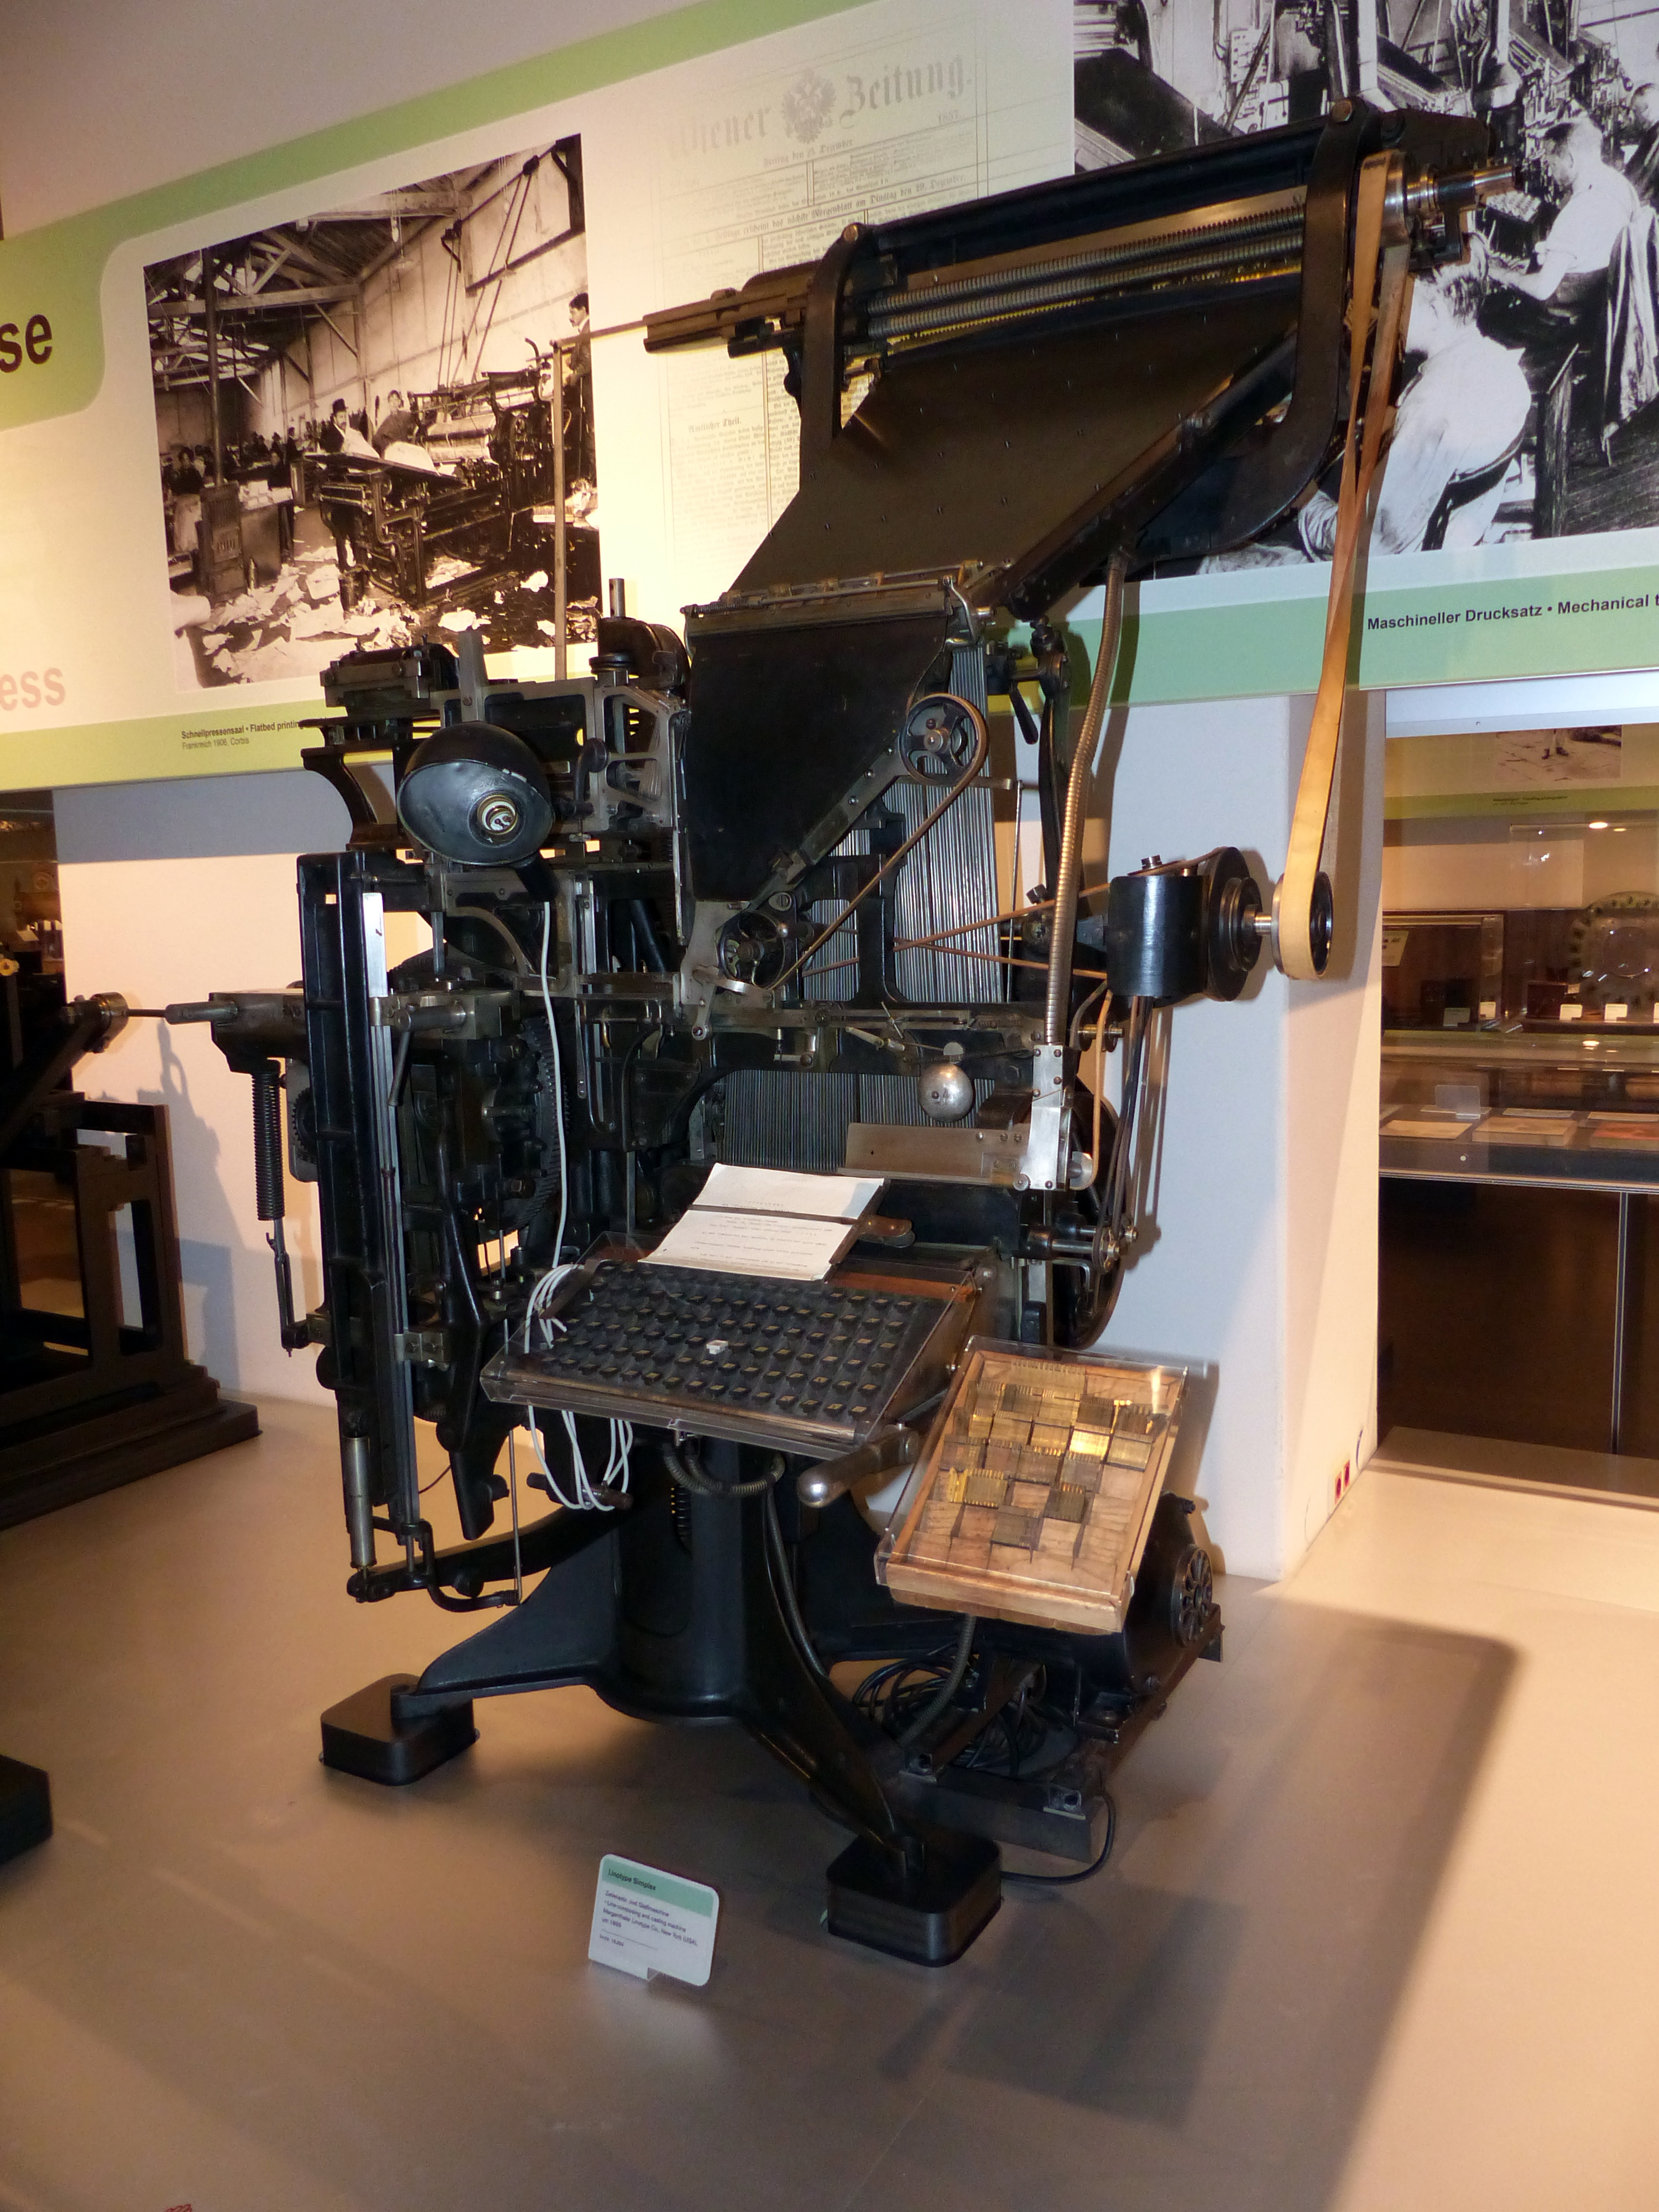
\includegraphics[width=0.45\textwidth]{figures/external/wikipedia_commons_Linotype_Simplex_1895}
    }
    \hfill
    \subfloat[First sub-figure\label{subfig-2:dummy}]{%
      \includegraphics[width=0.45\textwidth]{figures/external/public_domain_etaoin_shrdlu}
    }
    \caption{The origin of the name ``\abr{shrdlu}'': the most frequent
    letters on a linotype machine (left, a precursor to computerized word
    processors) which then became the title of a short story (right) of a
    machine that ingested the information it printed and became intelligent.}
    \label{fig:ir:linotype}
  \end{figure}


This machine becomes voracious, demanding
more and more input until the protagonist
%
of the story selectively feeds it Buddhist
philosophy and it achieves Nirvana.
%
Despite its funny name, SHRDLU remains the
OG question answering system.

The basic idea is that Instead of just answering
questions about a static world, you could
move objects around in this 3D world.
%
This is a later rendering of it … back in
the early 70s computer graphics aren’t as
advanced as they are today.

\jbgcomment{Add SHRDLU screenshot}

Wow, how far we’ve come.
%
And if the system couldn’t tell what object
you’re asking about (e.g., it’s ambiguous),
%
it asks a follow-up question to clarify which
one you meant.
%
I’m not going to go through the components
of SHRDLU, but it is fairly similar to LUNAR:
%
you parse sentences into a logical form.
%
The big difference is that the knowledge base
isn’t static: it changes as the user interacts
%
with the block world.

So there’s this part of the diagram that’s
unique to SHRDLU.
%
But I’m not going to talk about the details
of the implementation that much.
%
Why not?

Because you’ve probably noticed that these
systems are talking about narrower and narrower
%
domains.
%
They can just answer questions about baseball
games (not even baseball players), rocks from
%
the moon (not rocks generally, that’s too
much), and even SHRDLU goes further to build
%
its own world and only answering questions
about that.

And that goes back to the origin of the name
SHRDLU: taking text and making it into a reality
%
rather than understanding the world as it
is.
%
And the world as it is has ambiguity.

Let’s go back to the “Who’s on first
bit” that I started this video with.
%
So let me explain\footnote{At the risk of explaining the joke to much, there
are additional aspects that showcase the difficulties
in question answering.  
Pragmatics can be misinterpreted: ``I don't know'' can be a statement of fact
rather than saying that you \emph{lack} knowledge.  And grammar can be
critical in deciphering clues: ``I want to throw the guy at first base, so I
pick up the ball and throw it to Who'' makes it clear that ``who'' is a name,
while ``throw it to whom'' makes it clear that this is an interogative in the
objective case.} the Abbot and Costello routine:
there is a baseball player that has the name
%
``Who''.

Costello cannot figure out that “who”
is not an interrogative pronoun and never
%
interprets it as a proper noun.
%
Now, usually, that’s the right way to do
it.
%
But natural language is funny and ambiguous
sometimes.

And that’s the big difference between modern
QA systems and these older systems.
%
They’re small and brittle: when they work,
they work really well.
%
But they don’t work that often.

They’re not going to be able to handle random
questions from people on the Internet.
%
But that’s not to say that logic, semantic
parsing, and knowledge bases have no place
%
in 21st century question answering systems:
rather than taking a string of text and giving
%
a single answer, there are probabilistic interpretations
that provide a distribution over interpretations,
%
and then you train approaches using the Cranfield
paradigm to make sure that, yes, on average
%
it can answer the typical user’s questions.

\section{Leading up to Google}

And that's exactly the long-lasting legacy of the Cranfield paradigm shaped
 how we get answers from the internet.
 %
 For that, we need to leave central England and meet new player: NIST.  The
 American National Institute for Standards and Technology.

While the story of the birth of the Cranfield paradigm is an innovative
insight with Cyril Cleverdon combined with the vision of Karen Spärk Jones,
the story of NIST’s development of these test collections is one of slow,
methodological iteration.  Building up decades of expertise and slowly
building up bigger and better test collections, updating them each year so
that by the time Google’s PageRank came around, there’s no question about how
to tell whether a search engine is good enough.

Just fire up the latest test collection from the TREC conference, compute your precision and recall, and call it a day.
%
And this approach toward evaluation is with us in everything we do.  Test
collections are how we evaluate virtual assistants, question answering
systems, and just about every aspect of the modern Internet.  And it’s not
always for the best.  The ubiquity of these reusable test collections leads to
overfitting.  TREC puts out new datasets every year or so, but that’s not fast
enough for machine learning in the 21st century!  And while the focus on real
user data is good, the data you collect is biased by who is using technology
(mostly rich people from Western countries) and how they’ve been trained to
ask questions through decades of living with Cranfield-paradigm systems.  And
unlike people who work on, say, human-computer interaction, those building QA
systems often don’t actually put their system in front of real users.  And I
don’t think that’s what Cyril Cleverdon would have wanted.  His goal, as a
librarian, was to help users.  And yes, reusable test collections help you do
that—and they’ve spawned multibillion dollar companies around the world—but at
the end of the day you still need to check whether real users are actually
finding the information they need.

\jbgcomment{Citations for Google paper, examples}

\jbgcomment{Forward point to leaderboard chapter}
